\section{Experiment}

\subsection{Data}
To experiment our algoritm we use the dataset 20NewsGroup \cite{Newsgroups20}.
The 20 Newsgroups data set is a collection of approximately 20,000 newsgroup 
documents, partitioned evenly across 20 different newsgroups. We use also the 
RCV1 dataset \cite{Lewis:2004:RNB:1005332.1005345}. The RCV1 dataset is a 
collection of over 800,000 text documents. For RCV1 dataset, we use only a 
subset of 10,000 documents from RCV1 such that each document belongs to only 
one of the root classes in the class hierarchy. This was detailed in 
[\cite{Deap-K-Means}].\\
Each document are represented by a vector using term frequency-inverse document 
frequency (TFIDF) representation~\cite{doi:10.1108/eb026526}.
The term frequency-inverse document frequency is a method of weghting depicting 
the significance of each word of a document in relative to a corpus.
\begin{equation}
TF(t, X) = \frac{f_{t, X}}{max_{t' \in C}f_{t', X}} 
\end{equation}
\begin{equation}
IDF(t, C) = log(\frac{N}{|X \in C : t \in X|})
\end{equation}
\begin{equation}
TFIDF(t,X,C) = TF(t, X) . IDF(t, C)   
\end{equation}
For each dataset there is a preprocessing step. We remove stopword and keep only
the 2000 words with the top TFIDF scores. 
\subsection{Generate Constraint}
\subsubsection{Lexical Constraints}
To generate the set of keywords $KW$ we rank each word of each 
document of each class using TFIDF according to algorithm~\ref{algo:gen_kw}.
For our tests, we extract 3 keywords per classes.
\begin{algorithm}
  \SetKwInOut{Input}{input}
  \SetKwInOut{Output}{output}
  \Input{Corpus C, The number of keywords per classes $P$}
  \Output{KW}
  $KW \gets \{\}$\\
  \ForEach{Class $c_i \in C$}{
    $rank_i \gets [0 ... 0]$\\
    \ForEach{Document $X \in c_i$}{
      \ForEach{Word $w \in X$}{
        $rank_{i,w} \gets rank_{i,w} + TFIDF(w,X, C)$\\
      }
    }
  }
  \ForEach{Class $c_i, c_j \in C$}{
    \If{$c_i \neq c_j$}{
      $rank_i \gets rank_i - rank_j$\\
    }
  }
  \ForEach{Class $c_i \in C$}{
    $KW \gets KW \cup \{\{w_1, w_2 ... w_P\} : \not\exists (v_1, v_2) | v_1 \not\in 
    \{w_1, w_2 ... w_P\}, v_2 \in \{w_1, w_2 ... w_P\}, rank_{i,v_1} \ge rank_{i,v_2}\}$\\
  }
  \Return{KW}
  \caption{\label{algo:gen_kw}Extract Keywords}
\end{algorithm}
\subsubsection{Background Knowledge}
We generate pairwise constraints randomly accordinf to algorithm
~\ref{algo:gen_pair}
\begin{algorithm}[!h]
  \SetKwInOut{Input}{input}
  \SetKwInOut{Output}{output}
  \Input{Corpus C, The set of labels L, The number of pair $N_p$}
  \Output{Must-Link Pair ML, Cannot-Link Pair CL}
  \For{p = 1 : $N_p$}{
    \Repeat{$X_i \neq X_j \wedge L_i = L_j$}{
      Choose randomly ($X_i, X_j$)\\
    }
    Insert ($X_i, X_j$) in ML\\
  }
  \For{p = 1 : $N_p$}{
    \Repeat{$X_i \neq X_j \wedge L_i \neq L_j$}{
      Choose randomly ($X_i, X_j$)\\
    }
    Insert ($X_i, X_j$) in ML\\
  }
  \Return{ML, CL}
  \caption{\label{algo:gen_pair}Extract Pair}
\end{algorithm}
\subsection{Evaluation}
\subsubsection{Baseline Algorithm}
We evaluate our algorithm with Deep $K$-Means with pretraining see in section
~\ref{seq:DeepClust}.
\subsubsection{Metric}
To evaluate our algorithm and compare results with reference algorithms we can
use the NMI Metric, Accuracy Metric \cite{NMI_ACC}, and Adjusted
Rand index\cite{ARI}. 
\begin{itemize}
\item The NMI Metric is defined as follows
$$NMI(S,C) = \frac{I(S,C)}{[H(S)+H(C)]/2}$$ 
with
$I(S,C) =\sum_k \sum_f\frac{|s_k \cap c_f|}{N}log\frac{N|s_k \cap c_f|}{|s_k| |c_f|}$
and
$H(S) = -\sum_k\frac{|s_k|}{N}log\frac{N|s_k|}{|s_k|}$
\item The Accuracy is the proportion of true results among the total
  number of cases examined. The Accuracy metric is defined as follows :
$$
ACC(S,C) = \frac{1}{N}\sum_k {max}_j|s_k \cap c_j|
$$
\item Let a be the number of pairs of document in C
  that are in the same cluster in the predicted partition and in the
  same cluster in the real partition, and b be the number of pairs of
  document in C that are in different clusters in predicted partition
  and in different cluster in real partition.
  The Adjusted Rand index is defined as follows :
  $$ARI = \frac{a+b}{\binom{N}{2}}$$
\end{itemize}
\subsection{Experimental Setup}
\subsubsection{Autoencoder Architecture}
We use the same architecture used in~\cite{Deap-K-Means}. The encoder is a fully-connected 
multilayer perceptron formed by 3 hidden layers (with dimensions 500, 500, 2000) 
and an embedding layer (with dimension K, the number of cluster). 
The decoder is a mirrored version of the encoder~\ref{fig:archi}.
The ReLu activation function is used on layers, except for the third
hidden layer of encoder and decoder part.
\begin{figure}[!h]
  \centering
  \tikzset{every picture/.style={scale=1.6}}
  \fbox{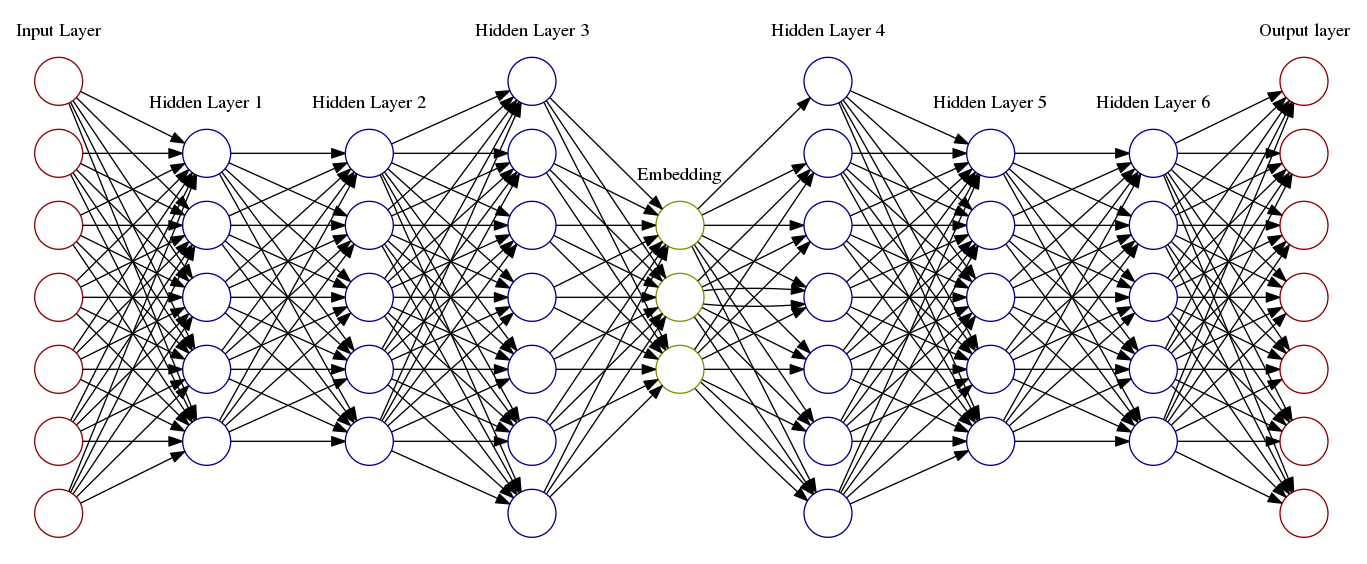
\includegraphics[scale=0.25]{parts/res/archi.png}}
  \caption{\label{fig:archi}Architecture}
\end{figure}
 
\subsubsection{Hyperparameters}
For the $\lambda$ hyperparameter we use the value defined in \cite{Deap-K-Means}. 
For the hyperparamter $\alpha_0$, we used Line Search~\cite{SWANN1969S39} strategy for 
$\alpha_0$ optimization. The Line search was done in two steps :
first, we searched on several range with 2 runs. Then we search on the range 
$[10^{-3},5.10^{-3},10^{-2},5.10^{-2},10^{-1}]$ with 5 runs.   
The results of Line Search are reported 
in table~\ref{tab:res}. Hyperparameters $alpha_1$, $alpha_2$ and $\eta$ 
are set to 0, because we focused on the lexical constraints in the experiments. 
\begin{table}[!h]
\centering
  \begin{tabular}{| l | l | l | l |}
    \hline
               & 20NEWS Without noise & 20NEWS With noise & RCV1 Without noise 
\\ \hline
    $\lambda$  & $10^{-1}$            & $10^{-1}$         & $10^{-2}$           
\\ \hline
    $\alpha_0$ & $10^{-2}$            & $5.10^{-3}$       & $10^{-1}$           
\\ \hline
  \end{tabular}
  \caption{\label{tab2}Best results of Line Search for the optimization of
hyperparameters for each dataset.}
\end{table}
\subsubsection{\label{section:test1}Clustering without Noise}
The purpose of the experiment is to rediscover the different classes of the
dataset with keywords and background knowledge.

\subsubsection{\label{section:test2}Clustering with Noise}
We divide the dataset into two corpus $C_1, C_2$. Each corpus contain
ten classes. We generate keywords \ref{algo:gen_kw} and pairwise
constraints \ref{algo:gen_pair} from $C_1$. Then we add noise to the corpus
$C_1$. To add noise, we concatenate document from corpus $C_1$ with document
from corpus $C_2$.
\\The purpose of the experiment is to rediscover the different classes of the
corpus $C_1$ with keywords and background knowledge.

\subsection{Results}
The results of these experiments are reported in table~\ref{tab:res}. We can  
observe that lexical constraints improve clustering's effectiveness. Then,
the most significiantly improve is for RCV1 dataset, this is because the number
of cluster for RCV1 is low. For the 20 newsgroup dataset, we can observe that 
the gain is higher when the data is noised, this is because lexical constraints
biaises representation toward a representation such that the significance of 
keywords is overestimated, and the rest of the document is underestimated.   

\begin{table}[!h]
\centering
  \begin{tabular}{| l | l | l | l | l | l | l | }
    \hline
    & \multicolumn{3}{|c|}{20NEWS Without noise} & \multicolumn{3}{|c|}{20NEWS With noise}  \\
    & ACC            &ARI             & NMI            & ACC           & ARI           &NMI            \\ \hline
Deep $K$-Means &$51.7\pm 1.9$&$33.6\pm 1.1$&$47.1\pm 0.9$&$42.8\pm 3.3$&$20.7\pm 1.9$&$28.3\pm 0.8$\\ \hline
Constrained Deep $K$-Means&\boldmath$53.4\pm 2.2$&\boldmath$35.4\pm 1.2$&\boldmath$47.4\pm 0.9$&\boldmath$45.3\pm 3$&\boldmath$23.23\pm 2.3$&\boldmath$30.0\pm 1.7$\\ \hline
  \end{tabular}
\begin{tabular}{| l | l | l | l | }
    \hline
     & \multicolumn{3}{|c|}{RCV1 Without noise}  \\
    &ACC            & ARI           &NMI  \\ \hline
Deep $K$-Means &$53.5\pm 3.4$&$24.1\pm 5.5$&$30.5\pm 5.3$
\\ \hline
Constrained Deep $K$-Means&\boldmath$62.7\pm 5$&\boldmath$31.7\pm 3.9$&\boldmath$37.2\pm 4$
\\ \hline
  \end{tabular}
\caption{\label{tab:res}Clustering with only lexical constraints applies to 
different learned latent space to measure the efficiency of lexical constraints
for $K$-Means algorithm. Performance is measured in terms of NMI, Adjusted Rand 
Index and clustering Accuracy, higher is better. Each cell contains the average
and the standard deviation computed over 5 run. The best result for each 
metric/dataset is underlined. In a first time, only lexical constraints have 
been tested. Homever, tests have been run on GPU server and seeds can't
be set, so the reproductibility is not guaranteed.}
\end{table}
